\section{Supervised and Unsupervised Learning}

\subsection{Supervised Learning1}
Supervised learning is a type of machine learning algorithm that uses a known dataset (called the training dataset) to make predictions. The training dataset includes input data and output data. The key of supervised learning is that you give your learning algorithm examples to learn from that include the "right answers", in other words the correct label \textbf{y} for the input \textbf{x}.
It learns by seeing correct pairs of inputs and outputs.  The goal is that eventually the algorithm will only be provided with the input-value(x) and it has to predict the output-value/label(y). 
Examples: \\ \\ \\

\begin{align*}
    \scalebox{1.3}{
\begin{tabular}{|c|c|c|}
    \hline
    Input(x) & Output(y) & Application \\
    \hline
    email & spam?(0/1) & spam filtering \\
    \hline
    audio & text transcript & speech recognition \\
    \hline
    English & Spanish & machine translation \\
    \hline
    ad,user,info & click?(0/1) & online advertising \\
    \hline
    image, radar info & position of other cars & self-driving car \\
    \hline
    image of a phone & defect?(0/1) & visual inspection \\
    \hline
\end{tabular}}
\end{align*}

In all of these applications you first train your model on data where you know the correct output. Then you use that model to make predictions on new data. \\

\subsubsection*{Regression: Housing Price Prediction}
Regression is a type of supervised learning algorithm that tries to predict a continuous output variable. In other words, it is used to predict a number. For example, predicting the price of a house in dollars is a regression problem whereas predicting whether a tumor is malignant or benign is a classification problem. \\
In other words, Regression is a type of algorithm that tries to predict a continuous output variable. 

\subsubsection*{Classification: Breast Cancer Prediction}
Say that you are trying to create a model that predicts whether or not a tumor is malignant or benign. In classification problems, the output variable is a category (such as "malignant" or "benign"). What we are trying to do is map input variables to discrete categories, we are classifying the input values into categories and trying to predict from the two possible output. Here we have a number of possible categories or outputs that our algorithm can predict. Whereas with regression we are trying to predict a continuous number. 
To summarise, Classification is a type of algorithm that tries to predict a discrete category, that doesn't necessarily have to be a number. Also in classification we are predicting a small set of possible outputs, so we are given our "options" in regards of what can our output be.
By extension obviously, we can have two or more inputs, in this case we can think of inputs as a "context" dataset that is provided to us, such as the tumor size, or the patient's age, sex, etc... The more context we provide the more accurate our prediction will be.
What we often do is represent our data-set in a function for example and our algorithm would try to identify some form of pattern in the data-set.

\subsection{Summary of Supervised Learning}
In summary supervised learning is when we are given a data-set and we are told what our correct output should be. We are given the "right answers" and we are trying to learn from that data-set to be able to predict the correct output for new data without the need of the input.
We have looked at two categories of supervised learning, regression and classification. In regression we are trying to predict a continuous number, and in classification we are trying to predict a discrete category.


\subsection{Unsupervised Learning}

Previously, in our classification problem what we have looked at is a supervised learning problem. We have a data-set and we are given the correct output(y) for each example. In unsupervised learning we are given a data-set but we are \textbf{not} given any labels or output value(y). Say you were given with the tumor size and the patient's age and any other context, however you don't know whether the tumor is malignant or benign. You are not given any labels or output value. 
Our job here is not to predict whether the tumor is malignant or benign, but rather to find some structure in the data-set. In other words find something interesting in the unlabeled data-set. 
The reason why it is called unsupervised is because we are not supervising the algorithm, we are not telling it what the correct answer is, we are just giving it the data and asking it to find some structure in the data.
So it might identify that the data can be divided into number of sections, or it might find some form of patterns between the patient's age and their tumor size, or any other contextual prediction.
Essentially it tries to place the data into different clusters, clustering is a type of unsupervised learning, where we are trying to find some structure in the data. For example clustering is used in google news. 
What google news does is every day it goes through all the news articles that are published and it tries to group them into different clusters, so that it can show you the different clusters of news articles and you can choose which cluster you are interested in.

Another type of unsupervised learning is anomaly detection where we are trying to find some abnormal behavior in the data. For example, if we have a data-set of credit card transactions and we are trying to find some unusual behavior in the data-set, such as unusual credit card transactions.
Another example is in manufacturing, where we are trying to find some unusual behavior in the manufacturing process, such as unusual defects in the product.
We also have dimensionality reduction where we are trying to take a data-set with a large number of features and reduce the number of features to a smaller number. For example, if we have a data-set with a large number of features, we might want to reduce the number of features to a smaller number so that we can visualize the data more easily.

\subsection{Linear Regression: House sizes and prices}
In this example let's imagine that we are given with a data-set about house prices and their sizes. We are given the size of the house in square feet and the price of the house in dollars. We are given a number of examples of houses and their prices. We are trying to predict the price of a new house given its size.
This is a perfect example of a linear regression model where we would first train our model on the data-set and showing the "right answers" and then we can use that model to predict the price of a new house given its size.

A data-set that is used to train a model is called a training set. The sizes of the house can be represented with x as for example if we  have a house that is 1000 square feet, we can represent that with x = 1000. The price of the house can be represented with y, so if the price of the house is 200,000 dollars, we can represent that with y = 200,000. 

We call x as the "input" variable or feature, and refer to y as the "output" variable or target. 

We can represent as a single training example by $$(x,y)$$ where x is the input and y is the output.
Our $i$th training example where I would represent a specific row from the training set would look like this: $(x^{(i)},y^{(i)})$.

Note that this doesn't mean that we are taking x and y to the power of i, but rather that we are taking the i'th training example from the training set.

So for example one example would look like this $$ (x^{(1)}, y^{(1)})=(2104,400) $$

Also as mentioned $$x^{(2)}\neq x^2$$

\subsection{Process of a Supervised training}
Supervised learning algorithm will input a dataset and then what exactly does it do and what does it output? 
Recall that a training set in supervised learning includes both the input features, such as the size of the house and also the output targets, such as the price of the house. The output targets are the right answers to the model we'll learn from.
To train the model, you feed the training set, both the input features and the output targets to your learning algorithm. Then your supervised learning algorithm will produce a function which we can call as $f$ that maps from x's to y's.
As every function this function will take an input x and then output a y which we can also call y-hat $\hat{y}$. So for example if we have a house that is 1000 square feet, we can input that into our function and it will output a price for that house.
y-hat in machine learning is the predicted output.
The function $f$ is called the "model". When we see only $y$ that is the actual output, when we see $\hat{y}$ that is the \textbf{predicted} output.
When designing the learning algorithm the question is that how do we choose the function $f$? What is the math formula that we are going to use? 
Inspired by the \textbf{slope-intercept form} $y=mx+b$ where $m$ is the slope and $b$ is the y-intercept, we can use the following formula for our function $f$:
$$ f_{w,b}(x) = wx + b $$ 
For now just note that both $w$ and $b$ are real numbers and will determine the prediction $\hat{y}$
Alternatively, we don't always have to include $w$ and $b$ we can simply just write $f(x)$ and it would be the same. 
We can represent the training set on a graph where our goal is to find the best fitting line using our function $f$.
We are using that function for future predictions, this process is what we call \textbf{Linear Regression with one variable} because we only have $x$ as the input which is the size of the house.
Now go through the model representation

\subsection{Cost Function}
The cost function will tell us how well the model is doing so that we can improve it and make sure that it's going to get better over time.
Recall that we have introduced our model: $$ f_{w,b}(x) = wx + b $$ and just to add a bit more terminology to it, we can call $w$ as the weights and $b$ as the bias.
Again this is what we call the slope-intercept form of a line, where $w$ is the slope and $b$ is the y-intercept.
For example if we were to have two points on a graph, let's say that we'd have the points (1,3) and (2,5) and we want to find the line that best fits these two points. We can use the slope-intercept form of a line to find the best fitting line.
First we have to find the slope, which is the change in y over the change in x, so we can calculate the slope as follows:
$$ m=\frac{\Delta x}{\Delta y}=\frac{y_2-y_1}{x_2-x_1}={\frac{5-3}{2-1}}=2 $$
Now that we have the slope we can find the y-intercept by using the following formula:
We can substitute the slope and one of the points into the formula to find the y-intercept:
$$ 3=2+b $$
$$ b=1 $$
So now we have the slope and the y-intercept, we can write the equation of the line as follows:
$$ y=2x+1 $$
Now this equation is the equation of the line that best fits the two points. We can plot the line on the graph and we can see that it fits the two points perfectly.
Obviously this was very easy and we also assumed that the line will go through these points, however this will not likely be the case in real life.
In real life we will have a lot more points and we will have to find the line that best fits all of these points. In order to do so we will have to use a cost function.
A cost function is a measure of how well a machine learning model performs by quantifying the difference between predicted and actual outputs.
In other words it will compute the difference between: $\hat{y}$ and $y$ as $\hat{y}-y$.
This difference is called the error, and we can also call it the loss. 
We can also square the error to make sure that it is positive, so we can write the error as follows:
\begin{align*}
    \scalebox{1.3}{$
    \sum_{i=0}^{m}\ (\hat{y}^{(i)}-y^{(i)})^2
  $}
\end{align*}
This case $m$ is the number of training examples, so we are summing over all of the training examples.
The problem here is that the more training examples we have, the larger the error will be. So we will have to divide the error by the number of training examples in order to avoid this huge numbers, so we can write the error as follows:
\begin{align*}
    \scalebox{1.3}{$
    \frac{1}{m}\sum_{i=0}^{m}\ (\hat{y}^{(i)}-y^{(i)})^2
  $}
\end{align*}

By convention machine learning people used to divide by $2m$, and also we can refer to the cost function as $J_(w,b)$ so our overall cost function will look like this:
\begin{align*}
    \scalebox{1.3}{$
    J_{(w,b)}=\frac{1}{2m}\sum_{i=0}^{m}\ (\hat{y}^{(i)}-y^{(i)})^2
  $}
\end{align*}

This is what we call the squared error cost function that is being used most commonly.

Now make sure to be aware of this: 
\begin{align*}
    \scalebox{1.3}{$
    J_{(w,b)}=\frac{1}{2m}\sum_{i=0}^{m}\ (f_w,b(x^{(i)})-y^{(i)})^2
  $}
\end{align*}

\subsection{More deeply about cost function}
We will use one example and actually get to see how the cost function can be used to find the best fitting line.
Now let's recap what we have so far.
\begin{enumerate}
  \item \textbf{model:} We have our \textbf{model} which is represented with the slope-interecept function: $f_w,b(x)=wx+b$ and depending on what values we choose for the slope $w$ and the y-interecept $b$ we are getting a line.
  \item  \textbf{parameters:} The model's parameters will $w$ and $b$, again our goal is to find the best values for $w$ $b$ to get the best fitting lines.
  \item \textbf{cost function:} Now in order to measure how good the values for $w$ and $b$ are we are using our cost function which we have constructed before: $$ J_{(w,b)}=\frac{1}{2m}\sum_{i=0}^{m}\ (f_w,b(x^{(i)})-y^{(i)})^2 $$ 
  We are taking the difference between the predicted value and the actual value for $y$, so we are trying to reduce the value of $J$
  \item \textbf{goal: } So we can say that our goal is to: $$ minimize J(w,b)$$
\end{enumerate}

Now let's see an example of how the cost function and the model would work. 
For simplicity we can get rid of the y-intercept $b$ meaning that our graphs will pass through the origin. 

\begin{align*}
  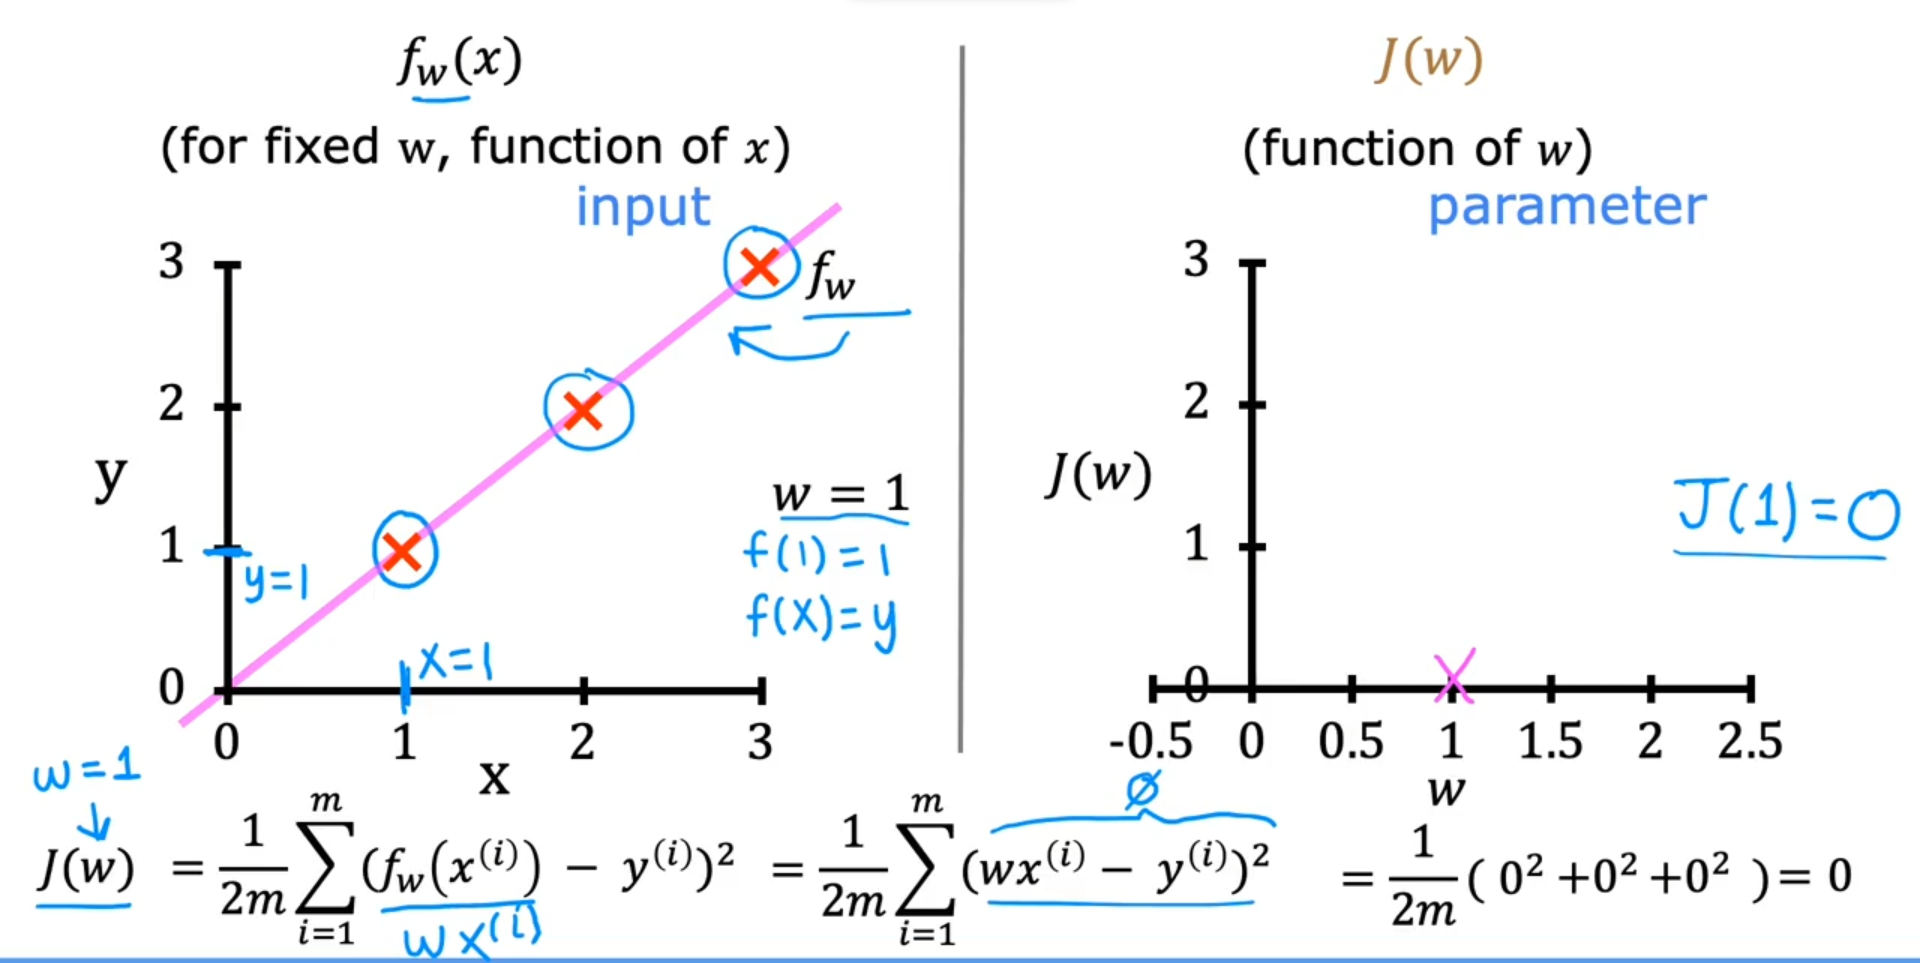
\includegraphics[width=1.2\textwidth]{machine-learning/andrew_ng_intro_to_ml/cost_function.png}
\end{align*}

As you can see here we have started off by plotting 3 points in which were: $(1,1)$ $(2,2)$ and $(3,3)$
Then what we wanted to do is test out our const function. We have identified the slope $w$ to be $1$ which ended up passing through all of the points perfectly. 
Since this line passes through all of the points we expected $J(x)$ to be 0. \\
Notice that when evaluating $J$ we are passing in the slope $w$ as the parameter. 
As you can see we have evaluated $J(w)$ and as we expected it turned out to be 0. 
In the other graph we can see that if we visualise the our slopes and const function solutions in a graph where we have the axis $w$ and $J(x)$.
We can see that when $w=1$ $J(x)=0$.
The reason why the cost function is zero, is because we have identified the slope of the function successfully which resulted the \textbf{perfectly} fitting line. 
We can validate our slope calculation by this formula: $$ m=\frac{\Delta y}{\Delta x}=\frac{1}{1}=1 $$ In short the slope is just a fraction of the change in y over the change in x.

Now let's try a different value of $w$ and pretend that we wouldn't know how to calculate the slope of this line.
If $w=0.5$ then obviously it's not going to fit the points well, therefore we expect $J(x)$ to be more than 0. 

\begin{align*}
  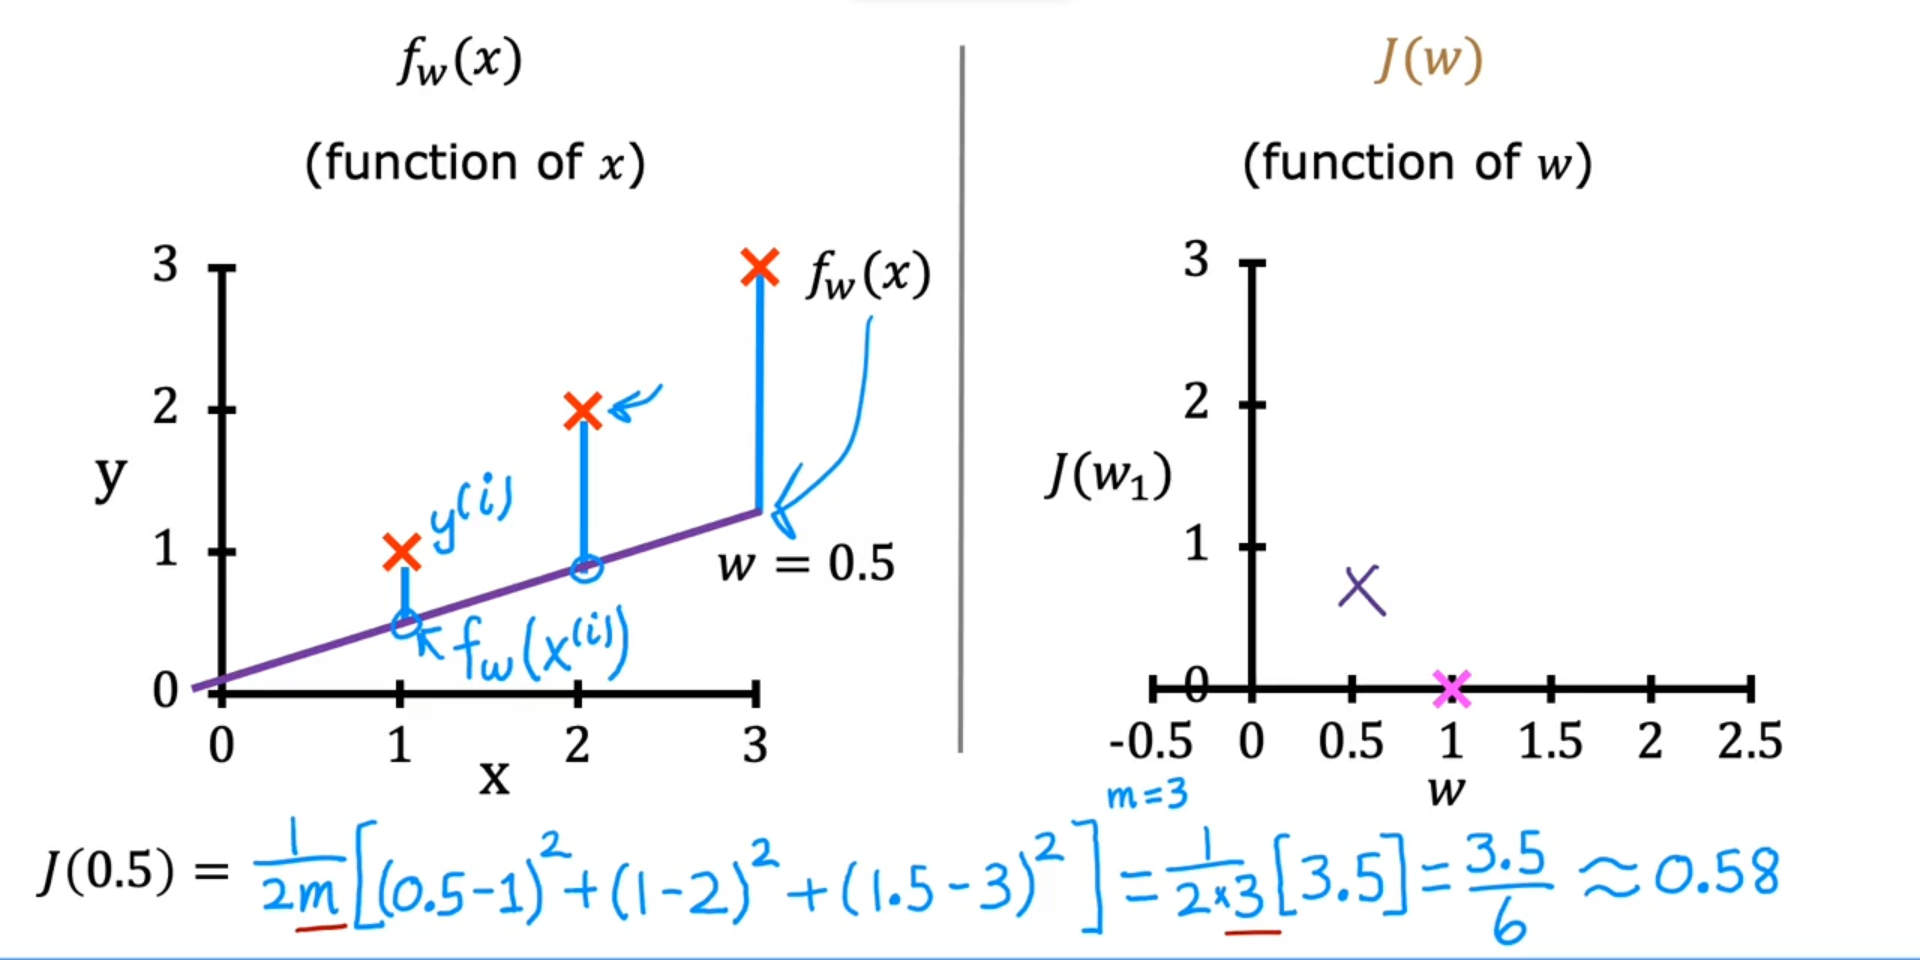
\includegraphics[width=1.2\textwidth]{machine-learning/andrew_ng_intro_to_ml/cost_function_0.5.png}
\end{align*}

We can see here that the line doesn't fit well to the points, therefore when calculating the difference between $\hat{y}-y$ and then square it we are actually going to get a number bigger than 0.
We can see that what we actually count by the difference $\hat{y}-y$ is the height from the predicted value to the actual value.  
When $w=0$ this is how it would look: 

\begin{align*}
  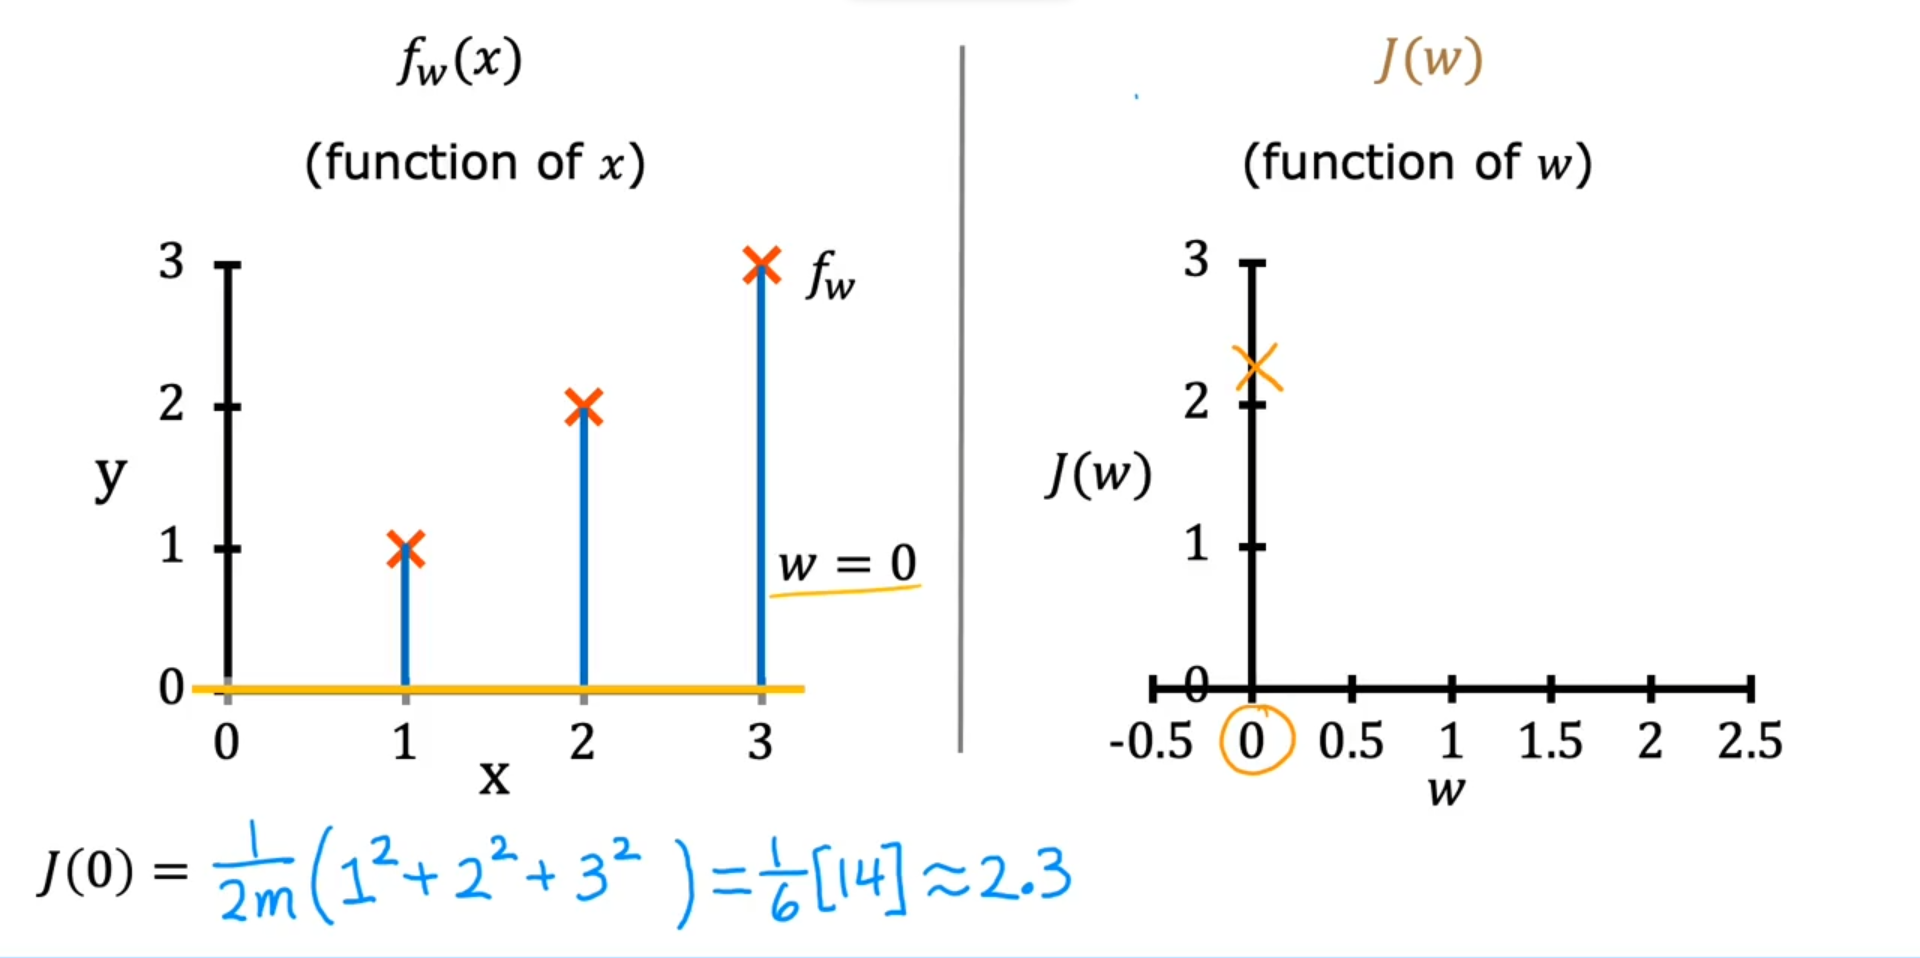
\includegraphics[width=1.2\textwidth]{machine-learning/andrew_ng_intro_to_ml/cost_function_0.png}
\end{align*}

We see that in this case since the slope of the line is $0$ and it has a y-intercept of 0, it's just going through the x-axis.
Obviosuly we could have had negative values for $w$ and then the cost function would have ended up being more, but in conclusion the further is the distance between the predicted and actual values the more the cost function is going to be.
If we keep going with the values we can see that the graph between $w$ and $J(w)$ turns out to be a curve. 

\begin{align*}
  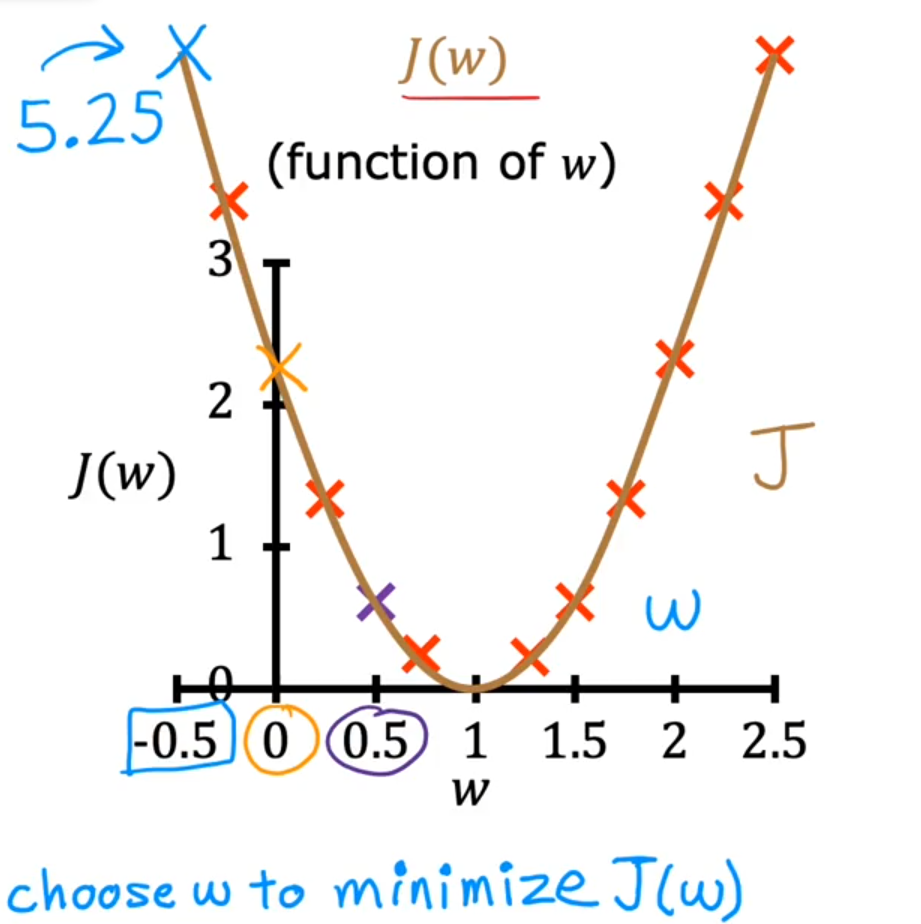
\includegraphics[width=1.2\textwidth]{machine-learning/andrew_ng_intro_to_ml/cost_function_slope_curve.png}
\end{align*}

This curve shows the different values of the cost function with their slopes. 
As we can see our goal was to have the smallest value of $J(w)$ and by our equation we concluded that when $J(w)=0$ will be $w=1$ which can be perfectly seen in the graph. 

This is how you can use the cost function to identify the best fitting slope $w$. 
Obviosuly we could have gotten further by having the y-intercept $b$ as a parameter but let's leave that to the next sections. 

In summary, we have conducted that the goal of linear regression is to choose values for $w$ and $b$ that results the cost function $J$ to be the smallest value possible. 

Now let's go through the model representation section 2 cost function